
\section{Analysis of the data}
Total implementation link for data analyzer : \\
\url{https://github.com/Sprea22/Data_Analyzer_Python}

During this part the main purpose is to analyse the whole dataset in order to find some kind of useful informations later on. \\
The Python system implemented in this section is mainly used for a generic analysis of the data from different point of views.\\
The output of this phase will basically be for each single data input:
\begin{itemize}
\item Total graphic of the input data from 2005 to 2016.
\item Graphic of the input data for each single year from 2005 to 2016.
\item Correlation matrix between different months of the same input.
\item Correlation matrix between different years of the same input.
\end{itemize}

And then it also provides:
\begin{itemize}
\item General correlation matrix between all the different inputs.
\item Graphic of the normalized angular coefficients of all the inputs.
\end{itemize}

It's important to remind that this phase can be implemented in different ways and with different programming language, in this case has been choose Python, so be sure to have installed all the necessary for compile and execute Python code on your platform.\\
Current development environment:\\
Python version: 2.7.12\\
Linux kernel version number: Linux Asus 4.4.0-71-generic SMP\\

During this experiment has been implemented a system that could be divided in two subsystems, that are:
\begin{itemize}
\item Single Input Analyzer (SIA): Used for analyze a single data input.
\item Multiple Inputs Analyzer (MIA): Used for analyze multiple data inputs.
\end{itemize}
\newpage


\newpage
\subsection{Single Input Analyzer}
\begin{itemize}
\item SIA imported libraries.
\item SIA part I: Generate and display a graphic about current input with total data from 2005 to 2016.
\item SIA part II: Generate and display a graphic about current input for each year from 2005 to 2016.
\item SIA part III: Generate and display a graphic that contains the correlation matrix between each single year from 2005 to 2016 of the current input.
\item SIA part IV: Generate and display a graphic that contains the correlation matrix between each single months of the year of the current input.
\item SIA part V: Generate and display a single overview image for the current input.
\end{itemize}

\subsubsection{Requirements for reusability}
The system that is going to be implemented in this phase of the work could be used for other data inputs as well, but there are of course some kind of requiriments about the dataset that are necessary for let it works in a proper way.\\
The aalysis system need in input a dataset structure that:
\begin{itemize}
\item Data from January 2005 to December 2016
\item One single value for each month
\end{itemize}
It means that the dataset must contains 144 values for each single input.
\newpage
\subsubsection{SIA: Imported libraries}
The "pandas" library will be very useful for read the data from CSV dataset and setup the plot abut it.
\begin{lstlisting}
import pandas as pd
\end{lstlisting}

The "numpy" library it's used for mathematic purpose, such as calculating the correlation coefficent between two series.
\begin{lstlisting}
import numpy as np
\end{lstlisting}
 
The "pyplot" library it's used for basic graphic displaying and customization, easy to use but very efficent.
\begin{lstlisting}
import matplotlib.pyplot as pyplot
\end{lstlisting}

Also the library "sys" would be very useful for test and execute the program, mainly because it allows to input directly from terminal.
\begin{lstlisting}
import sys
\end{lstlisting}

The library "PIL" supports many file formats, and provides powerful image processing and graphics capabilities.
\begin{lstlisting}
from PIL import Image
\end{lstlisting}

The library "fpdf" allows to generate and use PDF file.
\begin{lstlisting}
from fpdf import FPDF
\end{lstlisting}
\newpage
\subsubsection{SIA section I: Total graphic for all the years}
\textbf{Goal:}\\
Generate and display the total graphic about current input from 2005 to 2016.

\textbf{Requirements:}\\
- Data content: 144 values, 1 value for each month from 2005 to 2016

\textbf{Code implementation:}\\
During this section of the code was used "pandas" library for read the dataset.
\begin{lstlisting}
series = pd.read_csv("DATASET_DIRECTORY", header=0)
\end{lstlisting}

Then using the "pyplot" library has been possible to setup the plot of the input data.
\begin{lstlisting}
series.plot(color="blue", linewidth=1.5)
\end{lstlisting}


Thera are some settings about the axis x just to display the data in the right format, are easy to change and to costume.
\begin{lstlisting}
years = ["2005","2006","2007","2008","2009","2010",
	"2011","2012","2013","2014","2015","2016"]
x = range(144)
pyplot.xticks(np.arange(min(x), max(x)+1, 12.0), years)
pyplot.title("Total graphic from 2005 to 2016")
\end{lstlisting}

Once setted up the plot of the current data, the next step was to display the trendline of the current graphic. \\ 
The following code represent the method for calculate and display it.
\begin{lstlisting}
def trendline(x, y, col):
	z = np.polyfit(x, y, 1)
	p = np.poly1d(z)
	pylab.plot(x,p(x), c=col)
	# print "y=%.6fx+(%.6f)"%(z[0],z[1])
\end{lstlisting}	

At this point the current data values have been read again and passed to the method just impleneted above for calculating the trendline.
\begin{lstlisting}
seriesV = pd.read_csv("DATASET_DIRECTORY",header=0, 
		usecols=[1], squeeze=True)
trendline(x, seriesV.values, "red")
\end{lstlisting}

There is the possibility to save the graphic like an image and/or display it.
\begin{lstlisting}
pyplot.savefig("OUTPUT_DIRECTORY", format="jpg")
pyplot.show()
\end{lstlisting}

\begin{minipage}{0.5\textwidth}
\textbf{Results:} \\
With this first part of the code has been reached the first goal of to displaying and save the basic graphic about the current input from 2005 to 2016, with also the trendline displayed, that looks like this example:
\end{minipage} \hfill
\begin{minipage}{0.45\textwidth}
\begin{figure}[H]
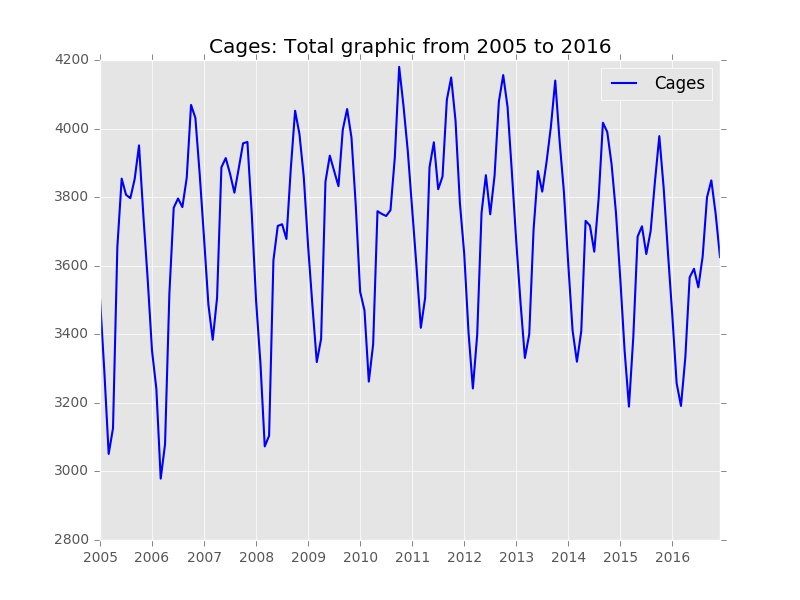
\includegraphics[width=0.9\textwidth]{Files/Cages_Total.jpg}
\caption{Total graphic about current input with total data from 2005 to 2016.}
\end{figure}
\end{minipage}


\newpage
\subsubsection{SIA section II: Single graphics for each year}

\textbf{Goal:}\\
Generate and display graphics about current input for each year from 2005 to 2016

\textbf{Requirements:}\\
- Data content: 144 values, 1 value for each month from 2005 to 2016

\textbf{Code implementation:}\\
During this section of the code was used "pandas" library for read the dataset.
\begin{lstlisting}
series2 = pd.read_csv("DATASET_DIRECTORY", 
	index_col=['Month'], 
	header=0, usecols=[0,1,2,3,4,5,6,7,8,9,10,11,12])
\end{lstlisting}

Then using the "pyplot" library has been possible to setup the plot of the input data.
\begin{lstlisting}
series2.plot()
\end{lstlisting}

Adding the title at the graphic that we are going to display.
\begin{lstlisting}
pyplot.title("Single year's graphic from 2005 to 2016")
\end{lstlisting}

There is the possibility to save the graphic like an image and/or display it.
\begin{lstlisting}
pyplot.savefig("OUTPUT_DIRECTORY", format="jpg")
pyplot.show()
\end{lstlisting}


\begin{minipage}{0.5\textwidth}
\textbf{Results:} \\
With this second part of the code has been reached the goal of displaying and save the graphics about the current input for each single year from 2005 to 2016, that looks like this example:
\end{minipage} \hfill
\begin{minipage}{0.45\textwidth}
\begin{figure}[H]
    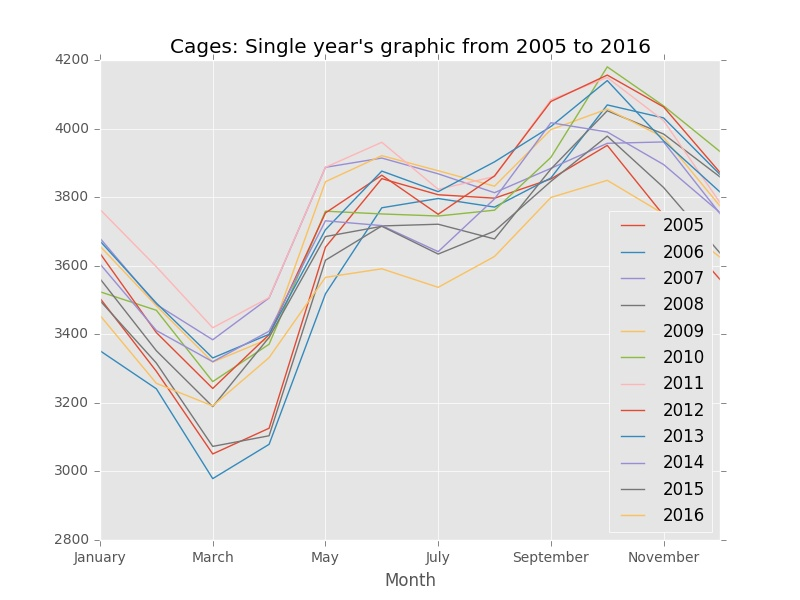
\includegraphics[width=0.9\textwidth]{Files/Cages_Years.jpg}
    \caption{Graphics for each single year of the input data from 2005 to 2016}
\end{figure}
\end{minipage}



\newpage
\subsubsection{SIA section III: Correlation matrix between years}

\textbf{Goal:}\\
Calculate the correlation coefficients between each single year from 2005 to 2016 of the current input and then display it with a correlation matrix.

\textbf{Requirements:}\\
- Data content: 144 values, 1 value for each month from 2005 to 2016

\textbf{Code implementation:}\\
During this section of the code was used "pandas" library for read the dataset.
\begin{lstlisting}
series3 = pd.read_csv("DATASET_DIRECTORY",
	 header=0, usecols=[1,2,3,4,5,6,7,8,9,10,11,12])
\end{lstlisting}

With the library "numpy" is possible to calculate the correlation coefficents between all the variables in the series just read.
\begin{lstlisting}
test = np.corrcoef(series3.values)
\end{lstlisting}

Setup the figure that will display the correlation matrix using the library "pypot".
\begin{lstlisting}
fig2 = pyplot.figure()
ax = fig2.add_subplot(111)
\end{lstlisting}

Creating the correlation matrix using the already calculated correlation coefficents.
\begin{lstlisting}
cax = ax.matshow(test, interpolation='nearest')
\end{lstlisting}

Settings for display the matrix in the right way, in particular for the values to display on both the axis x and y, in this case every single year from 2005 to 2016
\begin{lstlisting}
years = ["2005","2006","2007","2008","2009","2010",
	"2011","2012","2013","2014","2015","2016"]
x_pos = np.arange(len(years))
y_pos = np.arange(len(years))
pyplot.yticks(y_pos,years)
pyplot.xticks(x_pos,years)
\end{lstlisting}
\newpage
Adding a title to the graphic that we are going to display and also a bar that works like a legend for the colors of the matrix, allowing the reader to better understand the values reported inside the matrix.
\begin{lstlisting}
pyplot.title("Correlation between different years")
pyplot.colorbar(cax)
\end{lstlisting}

There is the possibility to save the correlation matrix like an image and/or display it.
\begin{lstlisting}
pyplot.savefig("OUTPUT_DIRECTORY", format="jpg")
pyplot.show()
\end{lstlisting}

\begin{minipage}{0.5\textwidth}
\textbf{Results:} \\
With this third part of the code have been calculated the correlation coefficients between each single year from 2005 to 2016 for each single inputs, saved the values in a document and then also displayed and saved the correlation matrix about it, that looks like this example:
\end{minipage} \hfill
\begin{minipage}{0.45\textwidth}
\begin{figure}[H]
    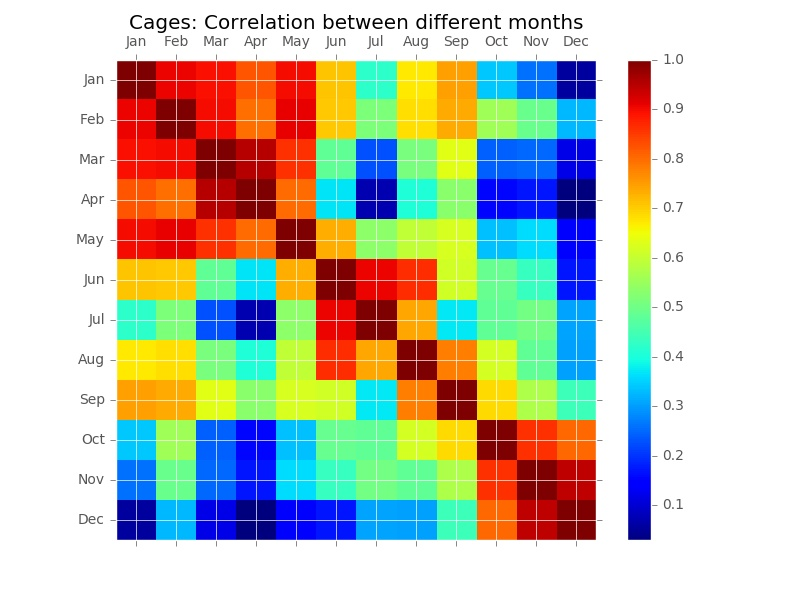
\includegraphics[width=0.9\textwidth]{Files/Cages_Months_Matrix.jpg}
    \caption{Correlation matrix between different months of the same input}
\end{figure}
\end{minipage}



\newpage
\subsubsection{SIA section IV: Correlation matrix between months}

\textbf{Goal:}\\
Calculate the correlation coefficients between each single month from 2005 to 2016 of the current input and then display it with a correlation matrix.

\textbf{Requirements:}\\
- Data content: 144 values, 1 value for each month from 2005 to 2016

\textbf{Code implementation:}\\
During this section of the code was used "pandas" library for read the dataset.
\begin{lstlisting}
series4 = pd.read_csv("DATASET_DIRECTORY", header=0, 
	usecols=[1,2,3,4,5,6,7,8,9,10,11,12])
\end{lstlisting}

With the library "numpy" is possible to calculate the correlation coefficents between all the variables in the series just read.
\begin{lstlisting}
test = np.corrcoef(series4.values)
\end{lstlisting}

Setup the figure that will display the correlation matrix using the library "pypot".
\begin{lstlisting}
fig2 = pyplot.figure()
ax = fig2.add_subplot(111)
\end{lstlisting}

Creating the correlation matrix using the already calculated correlation coefficents.
\begin{lstlisting}
cax = ax.matshow(test, interpolation='nearest')
\end{lstlisting}

Settings for display the matrix in the right way, in particular for the values to display on both the axis x and y, in this case every single months of the year.
\begin{lstlisting}
months = ["Jan","Feb","Mar","Apr","May","Jun",
	"Jul","Aug","Sep","Oct","Nov","Dec"]
x_pos = np.arange(len(months))
y_pos = np.arange(len(months))
pyplot.yticks(y_pos,months)
pyplot.xticks(x_pos,months)
\end{lstlisting}
\newpage
Adding a title to the graphic that we are going to display and also a bar that works like a legend for the colors of the matrix, allowing the reader to better understand the values reported inside the matrix.
\begin{lstlisting}
pyplot.title("Correlation between different months")
pyplot.colorbar(cax)
\end{lstlisting}

There is the possibility to save the correlation matrix like an image and/or display it.
\begin{lstlisting}
pyplot.savefig("OUTPUT_DIRECTORY", format="jpg")
pyplot.show()
\end{lstlisting}

\begin{minipage}{0.5\textwidth}
\textbf{Results:} \\
With this part of the code have been calculated the correlation coefficients between each single month from 2005 to 2016 of all the inputs and saved it in a document. Then has been also displayed and saved the correlation matrix about it, that looks like this example:
\end{minipage} \hfill
\begin{minipage}{0.45\textwidth}
\begin{figure}[H]
    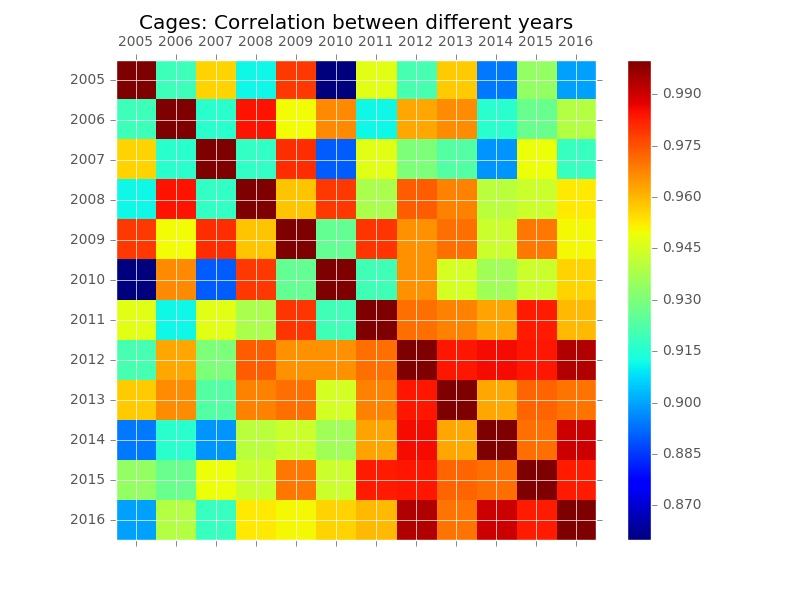
\includegraphics[width=0.9\textwidth]{Files/Cages_Years_Matrix.jpg}
    \caption{Correlation matrix between different years of the same input}
\end{figure}
\end{minipage}

\newpage
\subsubsection{SIA section V: Single and Total overview}

\textbf{Goal:}\\
Generate and display a single overview image for the current input.

\textbf{Requirements:}\\
- All the images that contain graphic about current input.

\textbf{Code implementation:}\\
create\_single\_overview() : this method will use the "Image" library for autogenerate a collage of the current input's graphics and save it like an overview image. The content of the params will basically decide how the "Current input overview image" will looks like.

It uses each single "current input overview image" of all the inputs and the "correlation matrix between all the inputs image" for combine them in a unique "total overview" and save it using the PDF format.

\begin{lstlisting}
listofimages=["CURRENT_INPUT_TOTAL_GRAPHIC",
            "CURRENT_INPUT_YEARS_MATRIX", 
            "CURRENT_INPUT_YEARS_GRAPHIC",
            "CURRENT_INPUT_MONTHS_MATRIX"]
           
create_single_overview(params1, listofimages)
create_single_overview(params2, listofimages)
\end{lstlisting}


The "create\_single\_overview" method has basically this structured, and then its configuration depends from the input data and from the preferences.
\begin{lstlisting}
def create_single_overview(cols, rows ,
			width, height, listofimages):
    thumbnail_width = width//cols
    thumbnail_height = height//rows
    size = thumbnail_width, thumbnail_height
    new_im = Image.new('RGB', (width, height))
    ims = []
    for p in listofimages:
        im = Image.open(p)
        im.thumbnail(size)
        ims.append(im)
    i = 0
    x = 0
    y = 0
    for col in range(cols):
        for row in range(rows):
            new_im.paste(ims[i], (x, y))
            i += 1
            y += thumbnail_height
        x += thumbnail_width
        y = 0
    new_im.save(SINGLE_OVERVIEW_IMAGE")
	new_im.show()
\end{lstlisting}

\textbf{Results:}
\begin{figure}[H]
	\centering
    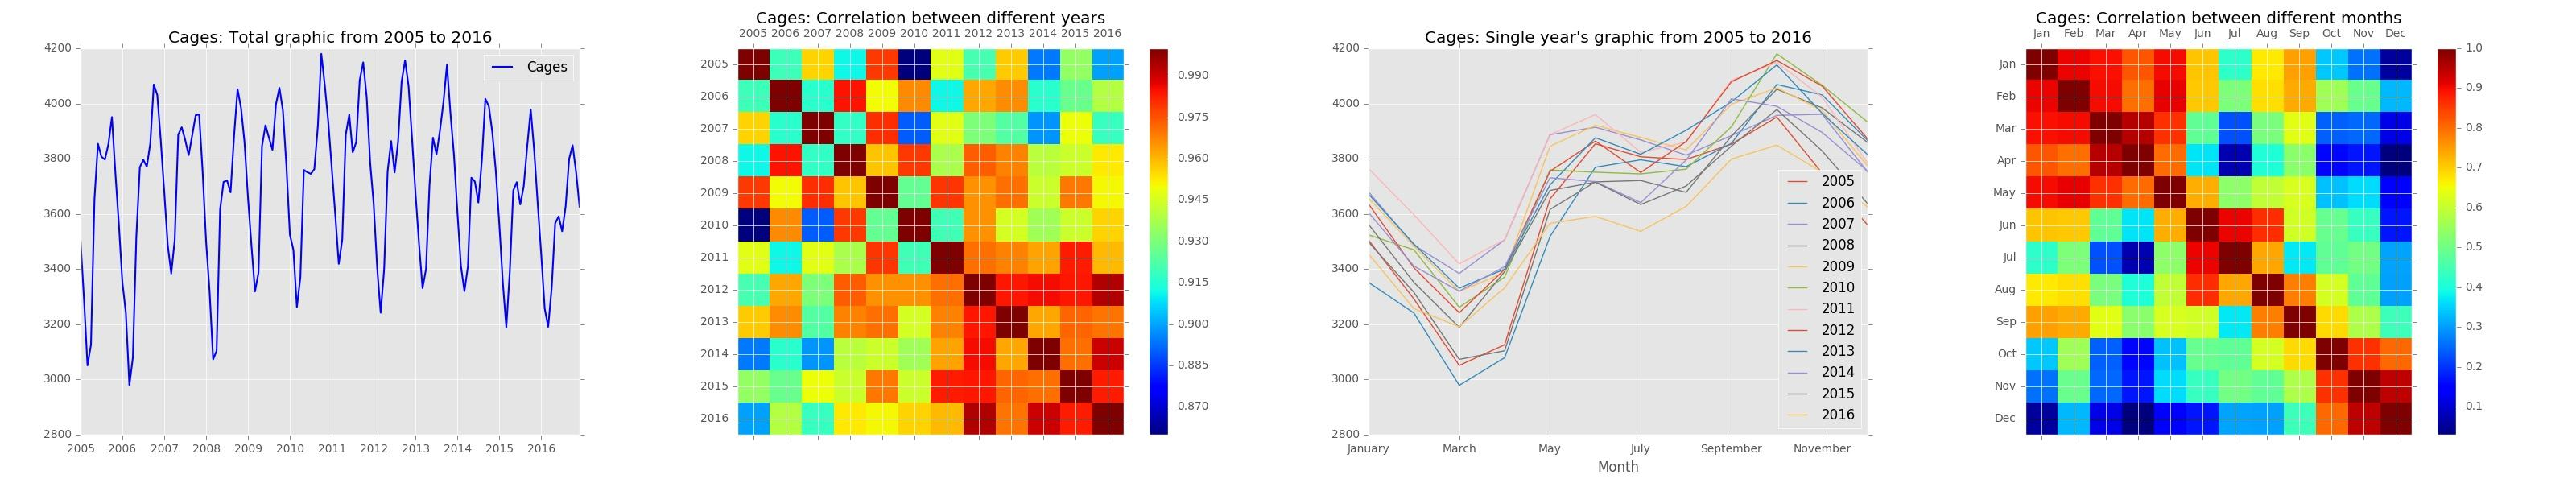
\includegraphics[width=1\textwidth]{Files/Cages_Overview.jpg}
    \caption{Example of "Single Input Overview Image"}
\end{figure}




\newpage
\subsection{Multiple Inputs Analyzer}
\subsubsection{MIA: Imported libraries}
The "pandas" library will be very useful for read the data from CSV dataset and setup the plot abut it.
\begin{lstlisting}
import pandas as pd
\end{lstlisting}

The "numpy" library it's used for mathematic purpose, such as calculating the correlation coefficent between two series.
\begin{lstlisting}
import numpy as np
\end{lstlisting}
 
The "pyplot" library it's used for basic graphic displaying and customization, easy to use but very efficent.
\begin{lstlisting}
import matplotlib.pyplot as pyplot
\end{lstlisting}

Also the library "sys" would be very useful for test and execute the program, mainly because it allows to input directly from terminal.
\begin{lstlisting}
import sys
\end{lstlisting}

\newpage
\subsubsection{MIA: Implementation}
\textbf{Goal:}\\
This analyzer is mainly used for show the correlation coefficent between the diffent inputs along the total period (from 2005 o 2016), that it will be important to have a general about which kind of relation there is between different inputs and how much strong it is.

\textbf{Requirements:}\\
- Input dataset: Total\_Dataset required, structure already reported here:
\hyperref[table: Total_Dataset]{Total Dataset}

\textbf{Code implementation:}\\
First of all, we are going to use the "pandas" library for read the dataset.
\begin{lstlisting}
series3 = pd.read_csv("TOTAL_DATASET_DIRECTORY", 
	index_col=['Input'], header=0)
\end{lstlisting}

Then with the library "numpy" is possible to calculate the correlation coefficents between all the variables just read above.
\begin{lstlisting}
test = np.corrcoef(series3.values)
\end{lstlisting}

Setup the figure that will display the correlation matrix using the library "pyplot".
\begin{lstlisting}
fig2 = pyplot.figure()
ax = fig2.add_subplot(111)
\end{lstlisting}

Creating the correlationg matrix using the already calculated correlation coefficents.
\begin{lstlisting}
cax = ax.matshow(test, interpolation='nearest')
\end{lstlisting}

Settings for display the matrix in the right way, in particular for the values to display on both the axis x and y, in this case every single input.
\begin{lstlisting}
inputs = ["Cages", "Feed", "Number", "Restock",
	"Local", "Withdr", "Biomass", "Price"]
x_pos = np.arange(len(inputs))
y_pos = np.arange(len(inputs))
pyplot.yticks(y_pos,inputs)
pyplot.xticks(x_pos,inputs)
\end{lstlisting}

Adding a title to the graphic that we are going to display and also a ba that works like a legend for the colors of the matrix, allowing the reader to better understand the values reported inside the matrix.
\begin{lstlisting}
pyplot.title("Correlation between different inputs 
		about data from 2005 to 2016")
pyplot.colorbar(cax)
\end{lstlisting}

In the end, using again the library "pyplot", there is the possibility to save the correlation matrix graphic like an image and/or display it.
\begin{lstlisting}
pyplot.savefig("OUTPUT_DIRECTORY")
\end{lstlisting}

\begin{lstlisting}
series = pd.read_csv("TRENDLINES_VALUES_DOCUMENT",
	 header=0, usecols=["Norm Ang Coeffs"])
series.plot(kind="barh")
pyplot.savefig("OUTPUT_DIRECTORY")

create_total_overview()
\end{lstlisting}

\begin{lstlisting}
pyplot.show()
\end{lstlisting}




\textbf{Results:} \\

\begin{figure}[H]
	\centering
    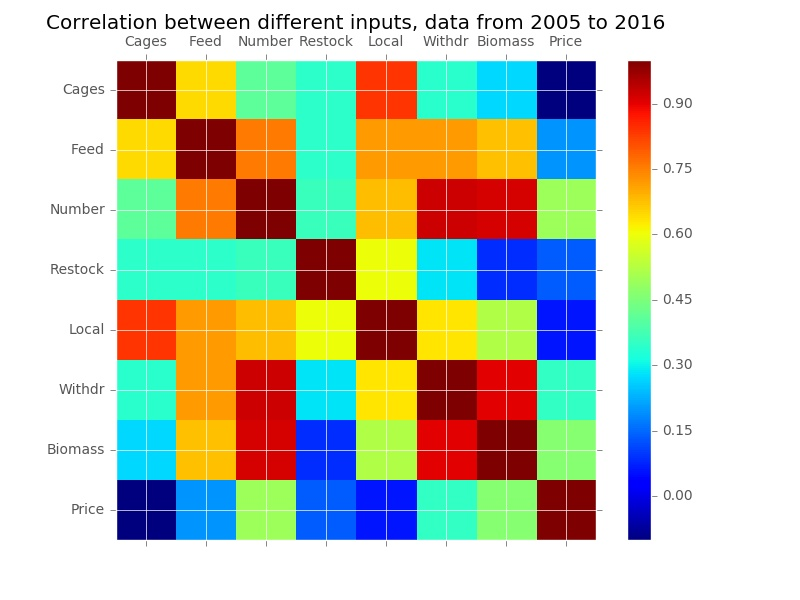
\includegraphics[width=0.75\textwidth]{Files/Total_Dataset_Years_Matrix.jpg}
    \caption{Correlation matrix between different inputs with data from 2005 to 2016.}
\end{figure}

\begin{figure}[H]
	\centering
    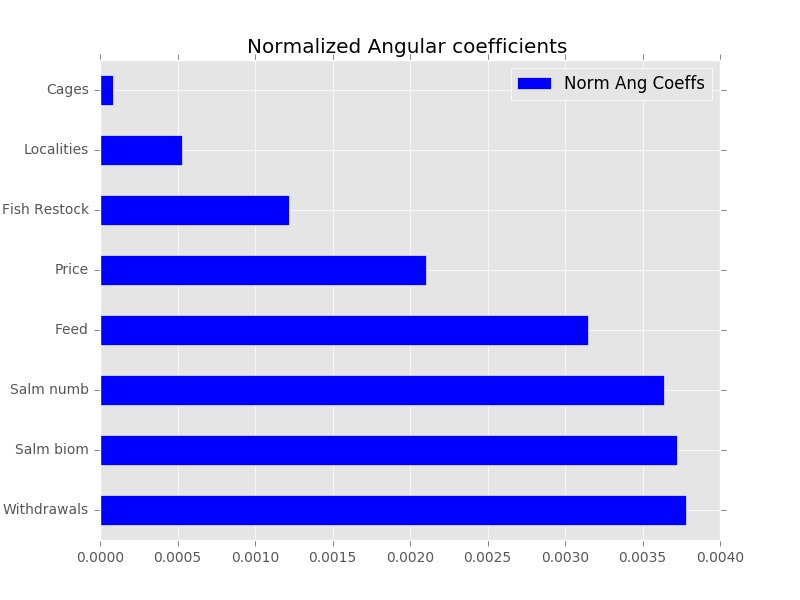
\includegraphics[width=0.75\textwidth]{Files/Norm_Ang_Coeffs.jpg}
    \caption{Normalized angular coefficients of each input's trendline.}
\end{figure}


\newpage
\section{Extract information from data}
